%%%%%%%%%%%%%%%%%%%%%%%%%%%%%%%%%%%%%%%%%
% baposter Landscape Poster
% LaTeX Template
% Version 1.0 (11/06/13)
%
% baposter Class Created by:
% Brian Amberg (baposter@brian-amberg.de)
%
% This template has been downloaded from:
% http://www.LaTeXTemplates.com
%
% License:
% CC BY-NC-SA 3.0 (http://creativecommons.org/licenses/by-nc-sa/3.0/)
%
%%%%%%%%%%%%%%%%%%%%%%%%%%%%%%%%%%%%%%%%%

%----------------------------------------------------------------------------------------
%	PACKAGES AND OTHER DOCUMENT CONFIGURATIONS
%----------------------------------------------------------------------------------------

\documentclass[landscape,a1paper,fontscale=0.6]{baposter} % Adjust the font scale/size here
\usepackage{mathtools}
\usepackage{graphicx} % support the \includegraphics command and options
\usepackage{caption}
\usepackage{subcaption}
\usepackage{wrapfig}
\usepackage[leftcaption]{sidecap}
\usepackage{lineno}
\usepackage{setspace}

\usepackage{graphicx} % Required for including images
\graphicspath{{figures/}} % Directory in which figures are stored

\usepackage{amsmath} % For typesetting math
\usepackage{amssymb} % Adds new symbols to be used in math mode

\usepackage{booktabs} % Top and bottom rules for tables
\usepackage{enumitem} % Used to reduce itemize/enumerate spacing
\usepackage{palatino} % Use the Palatino font
\usepackage[font=small,labelfont=bf]{caption} % Required for specifying captions to tables and figures

\usepackage{multicol} % Required for multiple columns
\setlength{\columnsep}{1.5em} % Slightly increase the space between columns
\setlength{\columnseprule}{0mm} % No horizontal rule between columns

\usepackage{tikz} % Required for flow chart
\usetikzlibrary{shapes,arrows} % Tikz libraries required for the flow chart in the template

\newcommand{\compresslist}{ % Define a command to reduce spacing within itemize/enumerate environments, this is used right after \begin{itemize} or \begin{enumerate}
\setlength{\itemsep}{1pt}
\setlength{\parskip}{0pt}
\setlength{\parsep}{0pt}
}

\definecolor{lightblue}{rgb}{0.145,0.6666,1} % Defines the color used for content box headers

\usepackage{graphicx}
\begin{document}

\begin{poster}
{
headerborder=closed, % Adds a border around the header of content boxes
colspacing=1em, % Column spacing
bgColorOne=white, % Background color for the gradient on the left side of the poster
bgColorTwo=white, % Background color for the gradient on the right side of the poster
borderColor=lightblue, % Border color
headerColorOne=black, % Background color for the header in the content boxes (left side)
headerColorTwo=lightblue, % Background color for the header in the content boxes (right side)
headerFontColor=white, % Text color for the header text in the content boxes
boxColorOne=white, % Background color of the content boxes
textborder=roundedleft, % Format of the border around content boxes, can be: none, bars, coils, triangles, rectangle, rounded, roundedsmall, roundedright or faded
eyecatcher=true, % Set to false for ignoring the left logo in the title and move the title left
headerheight=0.1\textheight, % Height of the header
headershape=roundedright, % Specify the rounded corner in the content box headers, can be: rectangle, small-rounded, roundedright, roundedleft or rounded
headerfont=\Large\bf\textsc, % Large, bold and sans serif font in the headers of content boxes
%textfont={\setlength{\parindent}{1.5em}}, % Uncomment for paragraph indentation
linewidth=2pt % Width of the border lines around content boxes
}
%----------------------------------------------------------------------------------------
%	TITLE SECTION 
%----------------------------------------------------------------------------------------
%
{\includegraphics[height=4em]{logo.png}} % First university/lab logo on the left
{\bf\textsc{Olfactory receptors are sensitive to molecular volume of odorants}\vspace{0.5em}} % Poster title
{\textsc{ Majid Saberi, \bf{Hamed Seyed-allaei} \vspace{0.5em} }}
{\includegraphics[height=4em]{logo.png}} % First university/lab logo on the 


%----------------------------------------------------------------------------------------
%	OBJECTIVES
%----------------------------------------------------------------------------------------

\headerbox{Objectives}{name=objectives,column=0,row=0}{
Which properties of a molecule define its odor? This is a basic question of olfaction, 
yet to be answered. Human olfactory system has a repertoire of about 350 olfactory receptors. 
Molecules bind to them with different affinities and activate them with different efficacies, 
resulting in a combinatorial code that identifies odorants. 
We hypothesized that the binding affinity between a pair of odorant-receptor is affected by their relative sizes. 
The affinity can reaches its maximum if molecular volume of an odorant matches volume of a receptor's binding-pocket 
and it reach zero if the sizes are too different, 
obscuring the effect of other molecular properties. 
We formulated this hypothesis mathematically and verified it on Data of Drosophila, 
and predicted the volume and the structural flexibility of each receptor’s binding-site, 
which are significantly different among receptors. 
This provides a reason for differences in smell among similar molecules of different sizes. 



\vspace{0.3em} % When there are two boxes, some whitespace may need to be added if the one on the right has more content
}

%----------------------------------------------------------------------------------------
%	INTRODUCTION
%----------------------------------------------------------------------------------------

\headerbox{materials and methods}{name=materilas and methods,column=1,row=0}{
DoOR database can be summarized in an $N\times M$ matrix. 
Its elements, $r_{nm}$, are the response of neuron $n$ to odorant $m$. 
This matrix is normalized between 0 and 1 so we have $0 \le r_{nm} \le 1$, where 1 is the strongest response.
The only problem is that this matrix has many {\it Not Available} (NA) values, 
and different neurons are excited by different set of odorants, 
so  when summing over $m$, $\sum_m$, we are calculating $\sum_{m: r_{nm} \neq \text{NA}}$, 
but for simplicity, 
we use the former notation. 

The response $r_{nm}$ depends on the molecular volume of the odorant, $v_m$, 
and other physio-chemical properties of the molecule $m$; 
We assume that we can separate the response $r_{nm}$ into two terms:

\begin{equation}
	r_{nm} = f_n(v_m) \psi_{nm}.
	\label{eqn:factors}
\end{equation}
The first term, $f_n(v_m)$, depends only on the molecular volume of odorants.
The second term, $\psi_{nm}$ include every other influential properties of molecules, but the molecular volume.
Both terms are characteristic of each receptor, and they might vary from neuron to neuron.
In fact, the first term, $f_n(v)$, is the tuning curve of neuron $n$ in respect to the molecular volumes, 
it can be approximated with a Gaussian function

\begin{equation}
	\displaystyle f_n(v) = e^{-\frac{(v-v_n)^2}{2\sigma^2_n}}, 
	\label{eqn:volume-dependence}
\end{equation}
where, $v_n$ is the preferred molecular volume of receptor $n$ and $\sigma_n$ represents its flexibility. 
In this work we want to estimate $v_n$ and $\sigma_n$. 
To do so, first we calculate the response weighted average of molecular volumes, 
$\frac{\sum_{m} v_m r_{nm}}{\sum_{m} r_{nm}}$ and then we use (\ref{eqn:factors}):

\begin{equation}
	\frac{\displaystyle \sum_{m} v_m r_{nm}}{\displaystyle \sum_{m} r_{nm}} = \frac{\displaystyle \sum_{m} v_m f_n(v_m) \psi_{nm}}{\displaystyle \sum_{m} f_n(v_m) \psi_{nm}}.
	\label{eqn:sta}
\end{equation}
Here we can approximate $\sum$ with $\int$, which is common in statistical physics:

\begin{equation}
	\sum_{m} \dots f_n(v_m) \psi_{nm} \approx  \langle \psi_{nm} \rangle_m \int_0^\infty \dots f_n(v) g(v)  dv. 
	\label{eqn:sigma_to_int}
\end{equation}
In which, 
$\langle \psi_{nm} \rangle_m$ denotes the average of $\psi_{nm}$ over all $m: r_{nm} \neq \text{NA}$. 
It can be moved out of the integral for it is independent of $v$.
In the above equation, 
$g(v)$ is the density of states, $g(v) dv$ indicates how many molecules have a molecular volume in the range of $v$ and $v+dv$.
This function can be approximated by a Gaussian function, Fig.\ref{fig:hist-volumes}, 

\begin{equation}
	g(v) = e^{-\frac{(v- v_{g})^2}{2 \sigma_{g}^2}},
	\label{eqn:hist-volumes}
\end{equation}
ideally, $g(v)$ should not depend on the neuron $n$, 
it is the property of ensemble of odorant molecules, not neurons. 
But here, we have many missing values ($r_{nm} = NA$), 
so we have to calculate $g(v)$ for each neuron separately; 
Therefore, $v_{g_n}$ and $\sigma_{g_n}$ are the average and standard deviation of molecular volume while $r_{nm} \neq \text{NA}$.
Now we rewrite equation (\ref{eqn:sta}) using equation (\ref{eqn:sigma_to_int}):

\begin{equation}
	\frac{\displaystyle \sum_{m} v_m r_{nm}}{\displaystyle \sum_{m} r_{nm}} \approx \frac{\displaystyle \int v f_n(v) g_n(v) dv}{\displaystyle \int f_n(v) g_n(v) dv}.
	\label{eqn:sta_int}
\end{equation}
We replace the product of $f_n(v)$ and $g_n(v)$ in the above equation with $h_n(v) = f_n(v) g_n(v)$, to make a simpler form

\begin{equation}
	\frac{\displaystyle \sum_{m} v_m r_{nm}}{\displaystyle \sum_{m} r_{nm}} \approx \frac{\displaystyle \int_v v h_n(v) dv}{ \displaystyle \int_v  h_n(v) dv }.
	\label{eqn:mean}
\end{equation}
The function $h_n(v)$ is a Gaussian function because it is the product of two Gaussian functions, 

\begin{equation}
h_n(v) = e^{-\frac{(v-\mu_{h_n})^2}{2\sigma_{h_n}^2}}, 
\end{equation}
so the right hand side of equation \ref{eqn:mean} is nothing but $\mu_{h_n}$ and 
in a similar way, we can calculate $\sigma_{h_n}$ from the neural data

\begin{eqnarray}
	\mu_{h_n} &\approx& \frac{\displaystyle \sum_{m} v_m r_{nm}}{\displaystyle \sum_{m} r_{nm}} \\
	\sigma_{h_n}^2 &\approx& \frac{\displaystyle \sum_{m} v_m^2 r_{nm}}{\displaystyle \sum_{m} r_{nm}} - \mu_{h_n}^2
	\label{eqn:final_h}
\end{eqnarray}•


We knew the mean $v_{g_n}$ and standard deviation $\sigma_{g_n}$ of $g_n(v)$ from the molecular volumes of the ensembles of odorants. 
We just calculated the mean $\mu_{h_n}$ and standard deviation $\sigma_{h_n}$ of $h_n(v)$ from the neural data.
Now calculating the mean $v_n$ and the standard deviation $\sigma_n$ of $f_n(v)$ is trivial,
first we calculate $\sigma_n$ from 

\begin{equation}
	\frac{1}{\sigma_n^2} = \frac{1}{\sigma^2_{h_n}}  - \frac{1}{\sigma^2_{g_n}}
\end{equation}•
and then we calculate $v_n$: 

\begin{equation}
	\frac{v_n}{\sigma_n^2}  =    \frac{\mu_{h_n}}{\sigma^2_{h_n}} - \frac{v_{g_n}}{\sigma^2_{g_n}}.
\end{equation}•

}

%----------------------------------------------------------------------------------------
%	RESULTS 1
%----------------------------------------------------------------------------------------

\headerbox{Results 1}{name=results,column=2,span=2,row=0}{

\begin{multicols}{2}
\vspace{1em}
\begin{center}
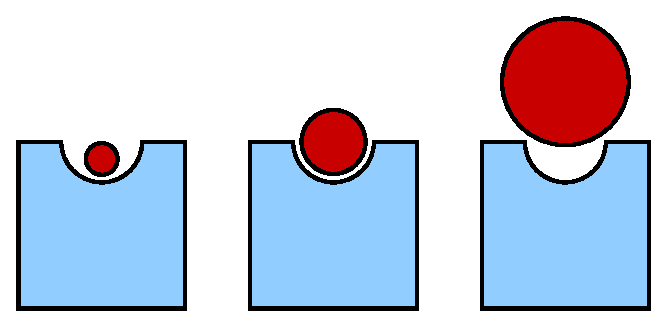
\includegraphics[width=0.8\linewidth]{binding-pocket}
\captionof{figure}{Figure caption}
\end{center}

Aliquam auctor, metus id ultrices porta, risus enim cursus sapien, quis iaculis sapien tortor sed odio. Mauris ante orci, euismod vitae tincidunt eu, porta ut neque. Aenean sapien est, viverra vel lacinia nec, venenatis eu nulla. Maecenas ut nunc nibh, et tempus libero. Aenean vitae risus ante. Pellentesque condimentum dui. Etiam sagittis purus non tellus tempor volutpat. Donec et dui non massa tristique adipiscing.
\end{multicols}

%------------------------------------------------

\begin{multicols}{2}
\vspace{1em}
Sed fringilla tempus hendrerit. Vestibulum ante ipsum primis in faucibus orci luctus et ultrices posuere cubilia Curae; Etiam ut elit sit amet metus lobortis consequat sit amet in libero. Lorem ipsum dolor sit amet, consectetur adipiscing elit. Phasellus vel sem magna. Nunc at convallis urna. isus ante. Pellentesque condimentum dui. Etiam sagittis purus non tellus tempor volutpat. Donec et dui non massa tristique adipiscing. Quisque vestibulum eros eu.

\begin{center}
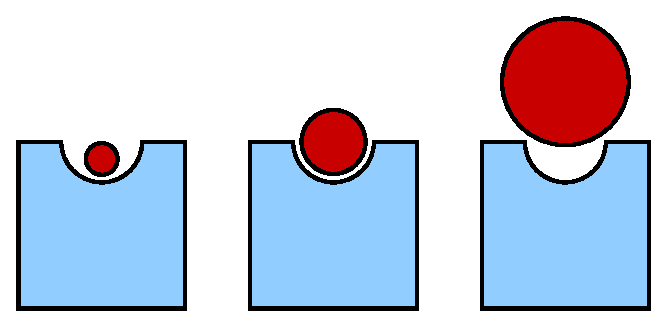
\includegraphics[width=0.8\linewidth]{binding-pocket}
\captionof{figure}{Figure caption}
\end{center}

\end{multicols}
}

%----------------------------------------------------------------------------------------
%	REFERENCES
%----------------------------------------------------------------------------------------

\headerbox{References}{name=references,column=0,above=bottom}{

\renewcommand{\section}[2]{\vskip 0.05em} % Get rid of the default "References" section title
\nocite{*} % Insert publications even if they are not cited in the poster
\small{ % Reduce the font size in this block
\bibliographystyle{unsrt}
\bibliography{sample} % Use sample.bib as the bibliography file
}}

%----------------------------------------------------------------------------------------
%	FUTURE RESEARCH
%----------------------------------------------------------------------------------------

\headerbox{Future Research}{name=futureresearch,column=1,span=2,aligned=references,above=bottom}{ % This block is as tall as the references block

\begin{multicols}{2}
Integer sed lectus vel mauris euismod suscipit. Praesent a est a est ultricies pellentesque. Donec tincidunt, nunc in feugiat varius, lectus lectus auctor lorem, egestas molestie risus erat ut nibh.

Maecenas viverra ligula a risus blandit vel tincidunt est adipiscing. Suspendisse mollis iaculis sem, in \emph{imperdiet} orci porta vitae. Quisque id dui sed ante sollicitudin sagittis.
\end{multicols}
}

%----------------------------------------------------------------------------------------
%	CONTACT INFORMATION
%----------------------------------------------------------------------------------------

\headerbox{Contact Information}{name=contact,column=3,aligned=references,above=bottom}{ % This block is as tall as the references block

\begin{description}\compresslist
\item[Web] www.university.edu/smithlab
\item[Email] john@smith.com
\item[Phone] +1 (000) 111 1111
\end{description}
}

%----------------------------------------------------------------------------------------
%	CONCLUSION
%----------------------------------------------------------------------------------------

\headerbox{Conclusion}{name=conclusion,column=2,span=2,row=0,below=results,above=references}{

\begin{multicols}{2}

\tikzstyle{decision} = [diamond, draw, fill=blue!20, text width=4.5em, text badly centered, node distance=2cm, inner sep=0pt]
\tikzstyle{block} = [rectangle, draw, fill=blue!20, text width=5em, text centered, rounded corners, minimum height=4em]
\tikzstyle{line} = [draw, -latex']
\tikzstyle{cloud} = [draw, ellipse, fill=red!20, node distance=3cm, minimum height=2em]

\begin{tikzpicture}[node distance = 2cm, auto]
\node [block] (init) {Initialize Model};
\node [cloud, left of=init] (Start) {Start};
\node [cloud, right of=init] (Start2) {Start Two};
\node [block, below of=init] (init2) {Initialize Two};
\node [decision, below of=init2] (End) {End};
\path [line] (init) -- (init2);
\path [line] (init2) -- (End);
\path [line, dashed] (Start) -- (init);
\path [line, dashed] (Start2) -- (init);
\path [line, dashed] (Start2) |- (init2);
\end{tikzpicture}

%------------------------------------------------

\begin{itemize}\compresslist
\item Pellentesque eget orci eros. Fusce ultricies, tellus et pellentesque fringilla, ante massa luctus libero, quis tristique purus urna nec nibh. Phasellus fermentum rutrum elementum. Nam quis justo lectus.
\item Vestibulum sem ante, hendrerit a gravida ac, blandit quis magna.
\item Donec sem metus, facilisis at condimentum eget, vehicula ut massa. Morbi consequat, diam sed convallis tincidunt, arcu nunc.
\item Nunc at convallis urna. isus ante. Pellentesque condimentum dui. Etiam sagittis purus non tellus tempor volutpat. Donec et dui non massa tristique adipiscing.
\end{itemize}

\end{multicols}
}

%----------------------------------------------------------------------------------------
%	Introduction
%----------------------------------------------------------------------------------------

\headerbox{introduction}{name=method,column=0,below=objectives,bottomaligned=}{ % This block's bottom aligns with the bottom of the conclusion block

%Survival of many species depends on their olfactory system. 
%They use it  to find food, 
%avoid poison, 
%escape from danger, 
%mate, 
%and bind to their offspring.
%An olfactory system detects volatile chemicals in the surrounding, 
%encodes the results and transmit them to limbic system and cortex.

%The front end of the olfactory system are olfactory receptor neurons.  
%Each neuron expresses only one kind of olfactory receptor (in insects they are co-expressed with Orco \cite{Larsson2004}).
%Neurons of the same type converge into the same glomeruli of the olfactory bulb (or antenatal lobe in insects),
%so that each glomerulus of olfactory bulb receives an amplified signal from only one type of olfactory receptor~\cite{root2007,Carey2011,Vosshall2000,Couto2005,fishilevich2005,gao2000,wang1998,mombaerts1996,vassar1994}.
%The olfactory systems use a combinatorial code: 
%unlike many other receptors which are activated by only specific ligands (eq. neurotransmitters and hormones),
%an olfactory receptor can be triggered by many odorant molecules, 
%and an odorant molecule can interact with different olfactory receptors~\cite{Malnic2000},

%The combinatorial code enables the olfactory system to discriminate trillion odors~\cite{Bushdid2014}.
%However, it is not clear yet which properties of a molecule contribute to its smell. It is a topic of ongoing researches and there are many theories~\cite{Turin,Keller2004,Araneda2000,Brookes2007,Franco2011,Pelz2006,Gabler2013,Schmuker2007,Haddad2008,Snitz2013,Yablonka2012,gane2013}.

%In this study, 
%we investigated the relation between molecular volumes of odorants and the responses of olfactory receptor neurons. 
%Our results suggest that molecular volume is a considerable factor, 
%but not the only factor that determines the neural response of the olfactory receptor neurons.

The olfactory receptors are transmembrane proteins.
In vertebrates, they are metabotropic receptors, they belong to the family of g-protein coupled receptor (GPCR). 
Linda B. Buck and Richard Axel won the Nobel Prize in Physiology or Medicine, in 2004, 
for its discovery ~\cite{Buck1991}.
There are many similarities between the olfactory system of insects and vertebrates~\cite{Wilson2014,Kaupp2010}, 
%and it was assumed that insects use the same kind of signal transduction~\cite{Brody2000,Hill04102002}. 
%But recently, it has been argued that the olfactory receptors in insects are inotropic~\cite{Sato2008,Wicher2008,Nagel2011,Rong2011}, 	
%their topology is different from vertebrates~\cite{Benton2007,Smart2008},
%and they function in presence of another common receptor, called Orco~\cite{Larsson2004}.
%Regardless of the signal transduction, 
all olfactory receptor have the same function, they have a binding-pocket (also known as binding-cavity and binding-site),
where the ligands (odorants) bind to. 
Binding to an odorant activates receptors and 
the activated receptors changes the potential of the cell, 
directly (inotropic) or indirectly (metabotropic).

The amount of change in the membrane potential of an olfactory receptor neuron depends on the number of activated olfactory receptor proteins and the time that they remain activated,
which are determined by various physio-chemical properties of the ligand (odorant) and the receptor~\cite{Turin,Araneda2000,Gabler2013,guerrieri2005,uchida2000}. 
But here we focus on two properties: the volume and the flexibility of the binding-pocket.
The molecular volume of a ligand should match the dimensions of the binding-pocket of the receptor,
then it fits into the binding-pocket of the receptor and triggers the signal transduction. 
Any mismatch in the volumes will affect the neural responses (Fig. \ref{fig:pocket-size}), 
on the other hand the flexibility of the binding-pocket can compensate for the volume mismatch (Fig. \ref{fig:pocket-flex}).

We could know the volume and flexibility of the binding-pocket, 
if we knew its three dimensional structure.
But this is not the case here, 
as it is not easy to know the structure of integral proteins~\cite{Zhang2008,Lupieri2009}, 
including olfactory receptors. 
%This is the topic of ongoing researches, 
%using various methods like Molecular Dynamic (MD) simulations, 
%mutagenesis studies, heterologus expression studies, and homology modeling~\cite{Khafizov2007,Man2004,Lai2005,Vaidehi2002,Floriano2004,Schmiedeberg2007,Katada2005,Kato2008,Rospars2013}.
In this study, we use neural recording to predict the {\it in-vivo} volume and flexibility of binding-pocket of olfactory receptors.

We suggest a functional relation between molecular volume and the neural responses, 
we provide a methodology to estimate {\it molecular receptive range} or {\it tuning function} of olfactory receptors,
and then we predict the structural properties of the binding-pocket of olfactory receptor - the volume and the flexibility of binding-pocket.
Our results may help to select odorants  for new experimental studies, 
may provide additional information about the structure of olfactory receptors to structural biologists, 
and may contribute to the study of olfactory coding.

To perform this study we use a public domain, 
well structured database -- DoOR -- 
that includes the neural responses of most olfactory receptors (OR) of Drosophila to many odorants~\cite{Galizia2010}. 
%This database aggregated data from many sources~\cite{Bruyne1999,Bruyne2001,Dobritsa2003,Goldman2005,Hallem2004,Hallem2006,
%Kreher2005,Kreher2008,Kwon2007,Pelz2006,Pelz2006,Schmuker2007,Stensmyr2003,
%Turner2009,VanderGoesvanNaters2007,Yao2005}.

%\begin{figure}
	\centering
%	\begin{subfigure}[b]{0.45 \textwidth}
		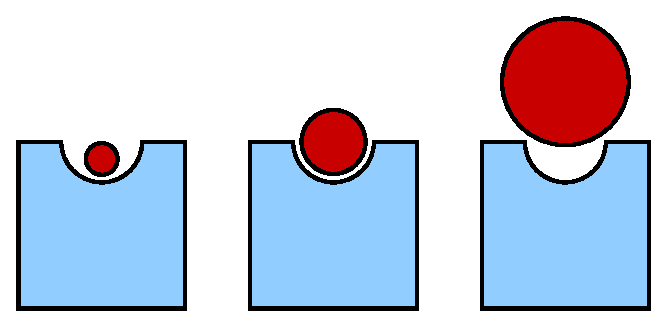
\includegraphics[width=10em]{binding-pocket}
%		\caption{Binding-pocket volume}
%		\label{fig:pocket-size}
%	\end{subfigure}
%	\hfill
%	\begin{subfigure}[b]{0.45 \textwidth}
		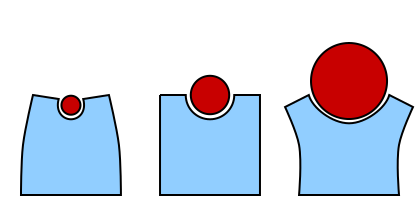
\includegraphics[width=10em]{binding-pocket-flex}
%		\caption{Binding-pocket flexibility}
%		\label{fig:pocket-flex}
%	\end{subfigure}
%	\caption{This figure shows different scenarios that may happen when an odorant molecule (ligand) binds to a receptor. 
%		Fig. \ref{fig:pocket-size} shows the effect of binding-pocket volume. 
%	From left to right, misfit because of small volume of molecule, perfect m%atch and misfit because of large molecular volume.
%		Fig. \ref{fig:pocket-flex} demonstrates that the flexibility of a receptor may compensate for the volume mismatches. 
%		The red disks (dark grey in b\&w) are odorant molecule, 
%		and the blue shapes (light grey in b\&w) are olfactory receptor and %binding-pocket.}
	\label{fig:binding-pocket}
%\end{figure}



}

\end{poster}

\end{document}